% F049: native TikZ/PGFPlots, computed from the stated mathematical model.
\begin{center}
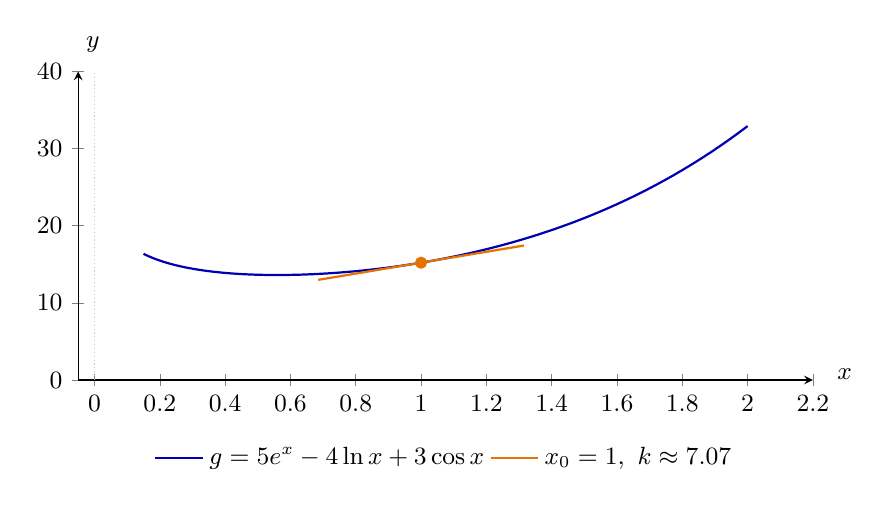
\begin{tikzpicture}[font=\small,>=stealth]
\begin{axis}[width=.90\linewidth,height=5.5cm,xmin=-0.05,xmax=2.2,ymin=0,ymax=40,
axis lines=left,xlabel={$x$},ylabel={$y$},font=\small,
xlabel style={at={(axis description cs:1.02,.02)},anchor=west},
ylabel style={rotate=-90,at={(axis description cs:.02,1.03)},anchor=south},
legend style={at={(axis description cs:.5,-.18)},anchor=north,draw=none,fill=none,font=\small,legend columns=2},
unbounded coords=jump,clip=true,]
\addplot[gray!45,thin,densely dotted,forget plot] coordinates {(0,0) (0,40)};
\addplot[blue!70!black,thick] coordinates {(0.15,16.363964) (0.16027778,16.154121) (0.17055556,15.961066) (0.18083333,15.782878) (0.19111111,15.617952) (0.20138889,15.464941) (0.21166667,15.322696) (0.22194444,15.190237) (0.23222222,15.066714) (0.2425,14.951393) (0.25277778,14.843628) (0.26305556,14.742855) (0.27333333,14.648574) (0.28361111,14.560341) (0.29388889,14.477762) (0.30416667,14.400483) (0.31444444,14.328188) (0.32472222,14.26059) (0.335,14.197432) (0.34527778,14.13848) (0.35555556,14.083521) (0.36583333,14.032362) (0.37611111,13.984828) (0.38638889,13.940756) (0.39666667,13.899999) (0.40694444,13.862421) (0.41722222,13.827898) (0.4275,13.796315) (0.43777778,13.767566) (0.44805556,13.741554) (0.45833333,13.718188) (0.46861111,13.697385) (0.47888889,13.679068) (0.48916667,13.663165) (0.49944444,13.64961) (0.50972222,13.638341) (0.52,13.629302) (0.53027778,13.622439) (0.54055556,13.617703) (0.55083333,13.615048) (0.56111111,13.614432) (0.57138889,13.615816) (0.58166667,13.619163) (0.59194444,13.62444) (0.60222222,13.631614) (0.6125,13.640656) (0.62277778,13.651541) (0.63305556,13.664242) (0.64333333,13.678736) (0.65361111,13.695003) (0.66388889,13.713024) (0.67416667,13.732779) (0.68444444,13.754253) (0.69472222,13.77743) (0.705,13.802298) (0.71527778,13.828843) (0.72555556,13.857056) (0.73583333,13.886925) (0.74611111,13.918442) (0.75638889,13.951599) (0.76666667,13.986389) (0.77694444,14.022807) (0.78722222,14.060848) (0.7975,14.100508) (0.80777778,14.141783) (0.81805556,14.184671) (0.82833333,14.229171) (0.83861111,14.275282) (0.84888889,14.323004) (0.85916667,14.372337) (0.86944444,14.423282) (0.87972222,14.475842) (0.89,14.53002) (0.90027778,14.585817) (0.91055556,14.643238) (0.92083333,14.702287) (0.93111111,14.76297) (0.94138889,14.82529) (0.95166667,14.889255) (0.96194444,14.954871) (0.97222222,15.022144) (0.9825,15.091082) (0.99277778,15.161693) (1.0030556,15.233984) (1.0133333,15.307966) (1.0236111,15.383646) (1.0338889,15.461034) (1.0441667,15.540141) (1.0544444,15.620977) (1.0647222,15.703552) (1.075,15.787879) (1.0852778,15.873967) (1.0955556,15.96183) (1.1058333,16.05148) (1.1161111,16.142929) (1.1263889,16.236191) (1.1366667,16.331279) (1.1469444,16.428206) (1.1572222,16.526987) (1.1675,16.627637) (1.1777778,16.730169) (1.1880556,16.8346) (1.1983333,16.940945) (1.2086111,17.049219) (1.2188889,17.15944) (1.2291667,17.271622) (1.2394444,17.385783) (1.2497222,17.50194) (1.26,17.620111) (1.2702778,17.740313) (1.2805556,17.862565) (1.2908333,17.986884) (1.3011111,18.113289) (1.3113889,18.2418) (1.3216667,18.372436) (1.3319444,18.505215) (1.3422222,18.640159) (1.3525,18.777287) (1.3627778,18.91662) (1.3730556,19.058178) (1.3833333,19.201984) (1.3936111,19.348057) (1.4038889,19.49642) (1.4141667,19.647096) (1.4244444,19.800105) (1.4347222,19.955472) (1.445,20.113218) (1.4552778,20.273367) (1.4655556,20.435943) (1.4758333,20.600969) (1.4861111,20.76847) (1.4963889,20.938469) (1.5066667,21.110992) (1.5169444,21.286064) (1.5272222,21.463711) (1.5375,21.643956) (1.5477778,21.826828) (1.5580556,22.012352) (1.5683333,22.200554) (1.5786111,22.391462) (1.5888889,22.585102) (1.5991667,22.781503) (1.6094444,22.980692) (1.6197222,23.182697) (1.63,23.387546) (1.6402778,23.595269) (1.6505556,23.805895) (1.6608333,24.019453) (1.6711111,24.235973) (1.6813889,24.455484) (1.6916667,24.678018) (1.7019444,24.903605) (1.7122222,25.132276) (1.7225,25.364062) (1.7327778,25.598996) (1.7430556,25.837109) (1.7533333,26.078433) (1.7636111,26.323003) (1.7738889,26.57085) (1.7841667,26.822008) (1.7944444,27.076511) (1.8047222,27.334392) (1.815,27.595688) (1.8252778,27.860432) (1.8355556,28.128659) (1.8458333,28.400406) (1.8561111,28.675708) (1.8663889,28.954601) (1.8766667,29.237123) (1.8869444,29.52331) (1.8972222,29.813199) (1.9075,30.106829) (1.9177778,30.404238) (1.9280556,30.705463) (1.9383333,31.010546) (1.9486111,31.319523) (1.9588889,31.632436) (1.9691667,31.949325) (1.9794444,32.27023) (1.9897222,32.595191) (2,32.924251)};
\addlegendentry{$g=5e^x-4\ln x+3\cos x$}
\addplot[orange!90!black,thick] coordinates {(0.685,12.986212) (1.315,17.43842)};
\addlegendentry{$x_0=1,\ k\approx7.07$}
\addplot[only marks,mark=*,orange!90!black,forget plot] coordinates {(1,15.212316)};

\end{axis}
\end{tikzpicture}
\par\smallskip{\small 按本题原函数绘图；切线斜率由本题的导函数计算。}
\end{center}
